\documentclass{article}
\usepackage{tikz,pgfplots,siunitx}

\newcommand{\imsize}{\linewidth}
\newlength\imagewidth% needed for scalebars
\newlength\imagescale% needed for scalebars
\newcommand{\ie}{i.\,e. }
\newcommand{\eg}{e.\,g. }

\begin{document}

To assess this claim, we additionally scanned a rat lung sample with four different protocols (A, B, C and D, details see Table~\ref{tab:abcd}). After acquisition of those four protocols, we artificially reduced the amount of projections of the central subscan. After merging these different sets of projections to in total 16 different datasets we reconstructed all those datasets for a more thorough analysis of the differences introduced through the reduction in amount of projections for the central subscan.

\begin{table}
	\centering
	\caption{Details of the protocols with artificially reduced amount of projections for the central scan to simulate influence of merging and interpolation.}
	\begin{tabular}{lcccclccc}
		Protocol & $\textrm{s}_{1}$ & $\textrm{s}_{2}$ & $\textrm{s}_{3}$ &  &  Protocol & $\textrm{s}_{1}$ & $\textrm{s}_{2}$ & $\textrm{s}_{3}$ \\
		A & 5040 & 5040 & 5040 &  &  B & 4536 & 4536 & 4536 \\
		A$\frac{\textrm{Central}}{2}$ & 5040 & 2520 & 5040 &  & B$\frac{\textrm{Central}}{2}$ & 4536 & 2268 & 4536 \\
		A$\frac{\textrm{Central}}{4}$ & 5040 & 1260 & 5040 &  & B$\frac{\textrm{Central}}{4}$ & 4536 & 1134 & 4536 \\
		A$\frac{\textrm{Central}}{8}$ & 5040 & 630 & 5040 &  & B$\frac{\textrm{Central}}{8}$ & 4536 & 567 & 4536 \\
		\hline
		C & 4032 & 4032 & 4032 &  &  D & 3528 & 3528 & 3528 \\
		C$\frac{\textrm{Central}}{2}$ & 4032 & 2016 & 4032 &  & D$\frac{\textrm{Central}}{2}$ & 3528 & 1764 & 3528 \\
		C$\frac{\textrm{Central}}{4}$ & 4032 & 1008 & 4032 &  & D$\frac{\textrm{Central}}{4}$ & 3528 & 882 & 3528 \\
		C$\frac{\textrm{Central}}{8}$ & 4032 & 504 & 4032 &  & D$\frac{\textrm{Central}}{8}$ & 3528 & 441 & 3528 \\
	\end{tabular}  
	\label{tab:abcd}
\end{table}

We assessed the structural similarity index \cite{Wang2004} of every 35\textsuperscript{th} slice of the dataset in comparison to the protocol with the maximal amount of acquired projections for this experiment (A)\footnote{The normalized error (as shown in Figure~\ref{fig:NormalizedErrorPlot}) has also been calculated and shows comparable results.}). As can be seen in Figure~\ref{fig:ssimplot}, the structural similarity index (SSIM) greatly decreases for a reduced amount of projections of the central subscan. Halving the projections of the central subscan reduces the SSIM for protocol A$\frac{\textrm{Central}}{2}$ (12600 total projections) lower than the quality of the unreduced protocol C (12096 total projections). Reducing the central subscan down to 630 projections (A$\frac{\textrm{Central}}{8}$, 10710 total projections), the quality of the reconstructions drops to the quality of the unreduced scan D (total 10584 projections). 

\begin{figure}
	\centering
		\caption{Plots of the mean SSIM parameter ($\pm$ Standard Deviation) for every 35\textsuperscript{th} slice for each of the protocols with artificially reduced central subscans}
		%\documentclass{article}
%\usepackage{tikz,pgfplots}
%\usepackage[pdftex,active,tightpage]{preview}
%\begin{document}
%\begin{preview}
%%%%%%%%%%%%
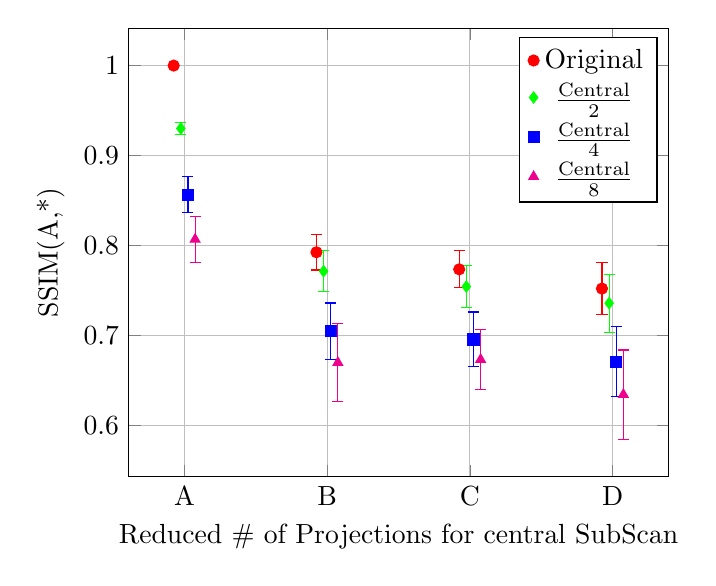
\begin{tikzpicture}

% Axis at [0.13 0.11 0.78 0.81]
\begin{axis}[
xmajorgrids,
ymajorgrids,
%axis on top,
%scale only axis,
%width=5.5cm,
%height=3.56562in,
%xmin=0.5, xmax=4.5,
%ymin=0.65, ymax=1,
xtick={1,2,3,4},
xticklabels={A,B,C,D},
xlabel={Reduced \# of Projections for central SubScan},
%title={mean SSIM for 25 Slices $\pm$ Std-Dev},
ylabel={SSIM(A,*)},
legend entries={Original,%
	$\frac{\textrm{Central}}{2}$,%
	$\frac{\textrm{Central}}{4}$,%
	$\frac{\textrm{Central}}{8}$}
]

\addplot [color=red, only marks, mark = * ]
plot[error bars/.cd, y dir = both, y explicit]
coordinates{
 (0.925,1) +- (0,0)
 (1.925,0.792335) +- (0,0.0197033)
 (2.925,0.773316) +- (0,0.0204757)
 (3.925,0.75192) +- (0,0.0287801)
};

\addplot [color=green, only marks, mark = diamond*]
plot[error bars/.cd, y dir = both, y explicit]
coordinates{
 (0.975,0.930057) +- (0,0.00648658)
 (1.975,0.771221) +- (0,0.0229399)
 (2.975,0.754166) +- (0,0.0237006)
 (3.975,0.735686) +- (0,0.0321475)
};

\addplot [color=blue, only marks, mark = square*]
plot[error bars/.cd, y dir = both, y explicit]
coordinates{
 (1.025,0.856407) +- (0,0.0197452)
 (2.025,0.704536) +- (0,0.0313107)
 (3.025,0.695346) +- (0,0.030527)
 (4.025,0.670378) +- (0,0.0388817)
};

\addplot [color=magenta, only marks, mark = triangle*]
plot[error bars/.cd, y dir = both, y explicit]
coordinates{
 (1.075,0.806686) +- (0,0.0254092)
 (2.075,0.669546) +- (0,0.0430564)
 (3.075,0.672877) +- (0,0.0333978)
 (4.075,0.633997) +- (0,0.0496304)
};

\end{axis}

\end{tikzpicture}
%%%%%%%%%%%%
%\end{preview}
%\end{document}%
	\label{fig:ssimplot}
\end{figure}

\renewcommand{\imsize}{.245\columnwidth}
\begin{figure}
	\centering
	\caption{Detailed view of ROI of one slice of protocol A and ROI of the same slice with artificially reduced central subscans (Aa, Ab and Ac). The ROI visible is cropped to the central part of the tomographic reconstruction, 512 pixels wide. Visible ripples are introduced for protocols Ab and Ac through the strong undersampling of the central subscan.}
	\pgfmathsetlength{\imagewidth}{\imsize}%
	\pgfmathsetlength{\imagescale}{\imagewidth/512}%
	\begin{tikzpicture}[x=\imagescale,y=-\imagescale]
		\def\x{316} % scalebar-x at golden ratio of x=512px
		\def\y{461} % scalebar-y at 90% of height of y=512px
		\node[anchor=north west, inner sep=0pt, outer sep=0pt] at (0,0) {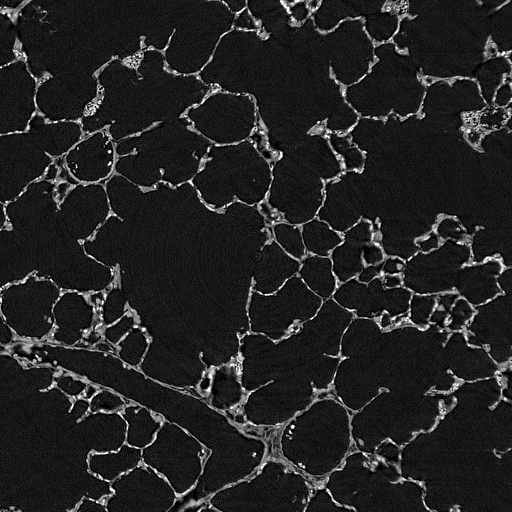
\includegraphics[width=\imagewidth]{img/ripples/R108C36B-A-mrg1024_rec_8bit.png}};
		% 513px = 0.75776mm > 100px = 148um > 338px = 500um, 68px = 100um
		%\draw[color=white,|-|,thick] (0,118) -- (512,117) node [sloped,midway,above] {\SI{0.75776}{\milli\meter} (512px)};
		\draw[color=white,|-|,thick] (\x,\y) -- (\x+136,\y) node [midway, above] {\SI{200}{\micro\meter}};
			\node [color=white, anchor=south west] at (0,512) {A};
			%\draw [color=white, thick] (0,512) rectangle (512,0);
		\end{tikzpicture}%
		\hfill%
		\begin{tikzpicture}[x=\imagescale,y=-\imagescale]
			\def\x{316} % scalebar-x at golden ratio of x=512px
			\def\y{461} % scalebar-y at 90% of height of y=512px
			\node[anchor=north west, inner sep=0pt, outer sep=0pt] at (0,0)
	    		{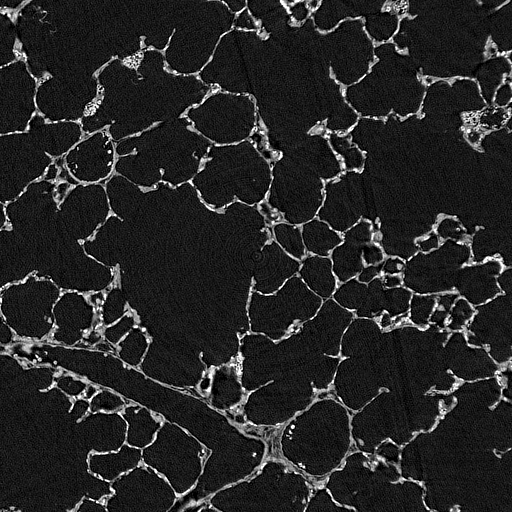
\includegraphics[width=\imagewidth]{img/ripples/R108C36B-Aa-mrg1024_rec_8bit.png}};
			% 513px = 0.75776mm > 100px = 148um > 338px = 500um, 68px = 100um
			%\draw[color=white,|-|,thick] (0,118) -- (512,117) node [sloped,midway,above] {\SI{0.75776}{\milli\meter} (512px)};
			\draw[color=white,|-|,thick] (\x,\y) -- (\x+136,\y) node [midway, above] {\SI{200}{\micro\meter}};
			\node [color=white, anchor=south west] at (0,512) {Aa};
			%\draw [color=white, thick] (0,512) rectangle (512,0);
		\end{tikzpicture}%
		\hfill%
		\begin{tikzpicture}[x=\imagescale,y=-\imagescale]
			\def\x{316} % scalebar-x at golden ratio of x=512px
			\def\y{461} % scalebar-y at 90% of height of y=512px
			\node[anchor=north west, inner sep=0pt, outer sep=0pt] at (0,0)
	    		{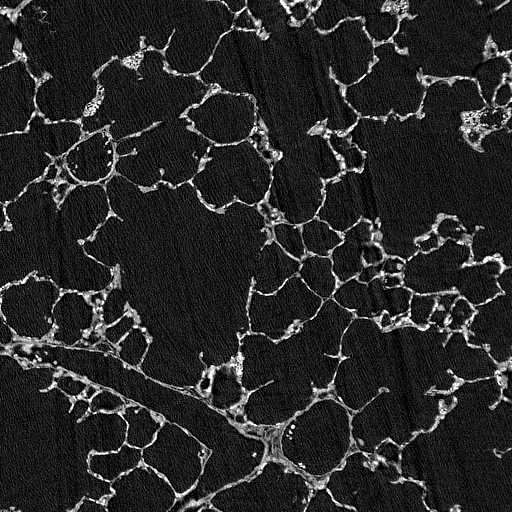
\includegraphics[width=\imagewidth]{img/ripples/R108C36B-Ab-mrg1024_rec_8bit.png}};
			% 513px = 0.75776mm > 100px = 148um > 338px = 500um, 68px = 100um
			%\draw[color=white,|-|,thick] (0,118) -- (512,117) node [sloped,midway,above] {\SI{0.75776}{\milli\meter} (512px)};
			\draw[color=white,|-|,thick] (\x,\y) -- (\x+136,\y) node [midway, above] {\SI{200}{\micro\meter}};
			\node [color=white, anchor=south west] at (0,512) {Ab};
			%\draw [color=white, thick] (0,512) rectangle (512,0);
		\end{tikzpicture}%
		\hfill%
		\begin{tikzpicture}[x=\imagescale,y=-\imagescale]
			\def\x{316} % scalebar-x at golden ratio of x=512px
			\def\y{461} % scalebar-y at 90% of height of y=512px
			\node[anchor=north west, inner sep=0pt, outer sep=0pt] at (0,0)
	    		{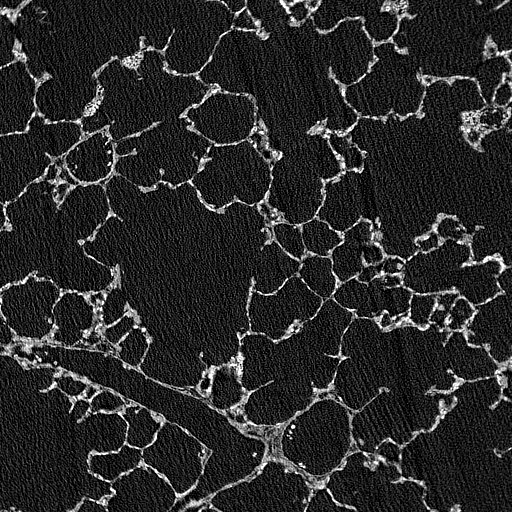
\includegraphics[width=\imagewidth]{img/ripples/R108C36B-Ac-mrg1024_rec_8bit.png}};
			% 513px = 0.75776mm > 100px = 148um > 338px = 500um, 68px = 100um
			%\draw[color=white,|-|,thick] (0,118) -- (512,117) node [sloped,midway,above] {\SI{0.75776}{\milli\meter} (512px)};
			\draw[color=white,|-|,thick] (\x,\y) -- (\x+136,\y) node [midway, above] {\SI{200}{\micro\meter}};
			\draw[color=white, anchor=south west] (0,512) node {Ac};
			%\draw [color=white, thick] (0,512) rectangle (512,0);
		\end{tikzpicture}%	
	\label{fig:ssim-details}
\end{figure}



\end{document}
